\subsection{Approximating NMF with STDPH}

That \ac{NSC} can explain and reproduce response properties observed in biological neurons may be an important clue as to how brains have evolved to parse and store information. One candidate \ac{NSC} process in the brain is synaptic plasticity
which, similar to \ac{NSC},
may act on synapses for the purpose of reducing dimensionality on an input space in order to represent it efficiently and sparsely.
Specifically, we propose that \ac{NSC} might be functionally equivalent to \ac{STDPH}
(Box 2).
\textbf{\Ac{STDP}} is a spike-timing based correlative learning rule in which the
timing of the pre- and post-synaptic spikes determine the amplitude and sign
of synaptic weight changes 
(i.e., long-term depression or long-term potentiation)
\citep{BiPoo1998,SongAbbott2000}.
Homeostasis acts to keep neuronal activity in a good working range,
acting across synapses of a single neuron and across multiple neurons
\citep{turrigiano1998}.
Whereas \ac{STDP} acts over a relatively short time scale (i.e., milliseconds to seconds),
homeostasis operates over minutes to days.
Homeostasis also facilitates synaptic competition by normalizing the inputs to a neuron. 
This evens the playing field for synapses that weaken due to imbalances in activity, 
but might otherwise strengthen if left to their own devices \citep{chistiakova2015}.

Experimental and theoretical evidence suggest that biological processes, such as synaptic plasticity and homeostatic mechanisms, may be reducing the dimensionality of inputs in a similar way to NMF. For example, Carlson and colleagues \citep{Carlson2013} delivered a mathematical proof
that \ac{STDPH} can approximate the \ac{NMF} algorithm (see Box 2).
Similar to Oja's rule \citep{Oja1982}, which was developed to stabilize 
rate-based Hebbian learning
(effectively resulting in \ac{PCA}),
synaptic scaling acts as a homeostatic mechanism to stabilize \ac{STDP}
(effectively resulting in \ac{NMF}).
This finding suggests that neurons are able to find accurate factorial
representations of their input stimulus spaces through means of Hebbian-like
synaptic learning. In addition, sparsity of the encoding might be enforced by spike thresholding \citep{Rozell2008}
and lateral inhibitory connections \citep{Coultrip1992}.

% \emilyNote{moved details to place where experiment is first described, but provide brief overview of STDPH and NMF experiment setups}
To investigate this equivalence
in a more realistic setting,
we conducted simulations in which a model constructed using \ac{STDPH}
and a model  constructed using \ac{NSC}
were applied to a dataset of recorded neuronal activity 
observed in the \ac{RSC} of rats in a  spatial navigation task 
(as shown for \ac{NSC} in Figure 1B3). 
In the \ac{STDPH} experiment, the idealized input neurons generated spike trains as input to a population of SNNs that were trained using an evolutionary strategy (Box 3) to match the recorded electrophysiological data \citep{Rounds2016}. In the \ac{NSC} experiment, the idealized neuronal output was used to construct a matrix of training data associated with each of the four recorded `features' (linear velocity, angular velocity, head direction, and position), to which \ac{NMF} was applied. 

% Half of the trials from each recording session in the dataset were used for training, while the latter half were reserved for testing. \emilyNote{said this in Box 3}
% \mikeNote{IMO these following paras are much too detailed. I think the EA details distract from the main argument, and don't add much value for the general understanding. The reader doesn't need to understand binary tournament selection, crossover, and mutation to appreciate the fact that you were able to fit SNN activity to neurophysiological recordings. Also now the glossary is 44\% EAs.}
% In these experiments, the
% \mikeNote{What population?}
% population size was $N = 15$. We randomly selected trials from a pool containing half the trials in the dataset for training (the other half were reserved for the testing phase). The testing phase was the same as the training phase except STDPH was disabled. Following testing, we measured correlations between synthetic and electrophysiological activity patterns and chose synthetic neuronal matches for each experimentally observed firing pattern based on the best correlations between them. Following fitness evaluation, we used
% \mikeNote{IMO could be shortened. ``We used an evolutionary strategy (binary tournament selection, mutation without crossover) implemented in CARLsim [REF] and ECJ [REF] to match this to that.'' or similar. }
% \textbf{binary tournament selection} to choose three new parents (each parent produced five children) for the next generation of individuals. Each new parent underwent mutation without crossover to produce a new child.
% To compare experimental neuronal responses with synthetic ones, we analyzed functional neuron types using methods described in Alexander and Nitz \citep{AlexanderNitz2015}. Activations averaged over trials for every neuron in the population were cross-correlated to reconstruct agent’s position within a route. To reconstruct position with respect to one route (such as in 
% \mikeNote{Please first explain what $\alpha$ and $\beta$ are. L and R are a bit easier to guess}
% $\alpha$LRL), trials were divided into two sets, even and odd, to measure consistency of response. To reconstruct position between track positions (such as in $\alpha$$\beta$LRL), activations over trials associated with the $\alpha$ track position were averaged and cross-correlated with averaged activations over trials associated with $\beta$. High correlations between same positions (e.g., bin 1 (row) and bin 1 (column)) indicate a good reconstruction of position from ensemble activity
% \mikeNote{add ``see Fig. X, Y'' etc.?}
% patterns. Within-position reconstructions (even vs. odd trials) yielded accurate positional reconstructions (low error), but between-position (i.e., $\alpha$ vs. $\beta$ trials) were associated with high error and did not yield accurate reconstructions of position, which suggests that the population differentiates routes situated in different parts of space.
% The evolutionary algorithm was used to optimize STDPH parameters in the model, corresponding to the temporal window over which spike times were integrated, the amount each synaptic weight increased or decreased, and the target baseline firing rates of excitatory and inhibitory neurons. During each generation of the evolutionary run, models were trained on trials randomly selected from half of the available dataset, then tested on trials randomly selected from the latter half reserved for testing. At the end of each generation, synthetic neural activity was correlated with electrophysiologically recorded neural activity, which served as the fitness metric for the algorithm. After the model finished an evolutionary run, SNN activity closely matched the electrophysiological activity. For the \ac{NSC} experiment, we constructed an input matrix containing half the trials associated with the task to be used as a training set, in which each row was one of the four behavioral metrics, and each column was associated with an element in one of the recorded trials. We applied \ac{NMF} to the input matrix and then used the remaining half of the trials to test the model and gather responses from the model neurons.

We found that the activity patterns of both \ac{NSC} and \ac{STDPH} model neurons could replicate the neuronal response properties and ensemble activity seen in the electrophysiologically recorded neurons in the dataset (Fig.~\ref{fig:NMF|RSC}A, B, C, left); that is, the model neuron activity could be classified into three broad categories,
with remarkably similar population statistics to rat \ac{RSC} 
\citep{AlexanderNitz2015}:
1) Turn-sensitive, no modulation neurons responded whenever the animal made a left or right turn
   on the track (light gray);
2) Turn-sensitive, route modulation neurons responded whenever the animal made a turn on a specific position along
   the route, independent of allocentric location (dark gray); and
3) Turn-insensitive neurons that could not be classified according to the above,
   but nonetheless exhibited complex and robust firing patterns (white). In addition, both \ac{NSC} and \ac{STDPH} model \ac{RSC} produced simulated neurons whose ensemble activity vectors could be used to predict the agent's location on a route with respect to the allocentric frame of reference. Ensemble activity patterns could also disambiguate the agent's location within routes that occupied different locations in the room, consistent with findings of population behavior in the biological RSC \citep{AlexanderNitz2015}.
When even and odd trials on the same track locations were compared,
ensemble prediction error was very low,
but when the tracks were in two different locations
(i.e., $\alpha$ vs. $\beta$),
the prediction error was significantly higher in all cases
(Fig.~\ref{fig:NMF|RSC}A, B, C, right).
For further details on this analysis, see \citep{AlexanderNitz2015,Rounds2016}.
   
\begin{figure}[ht]
	\centering
	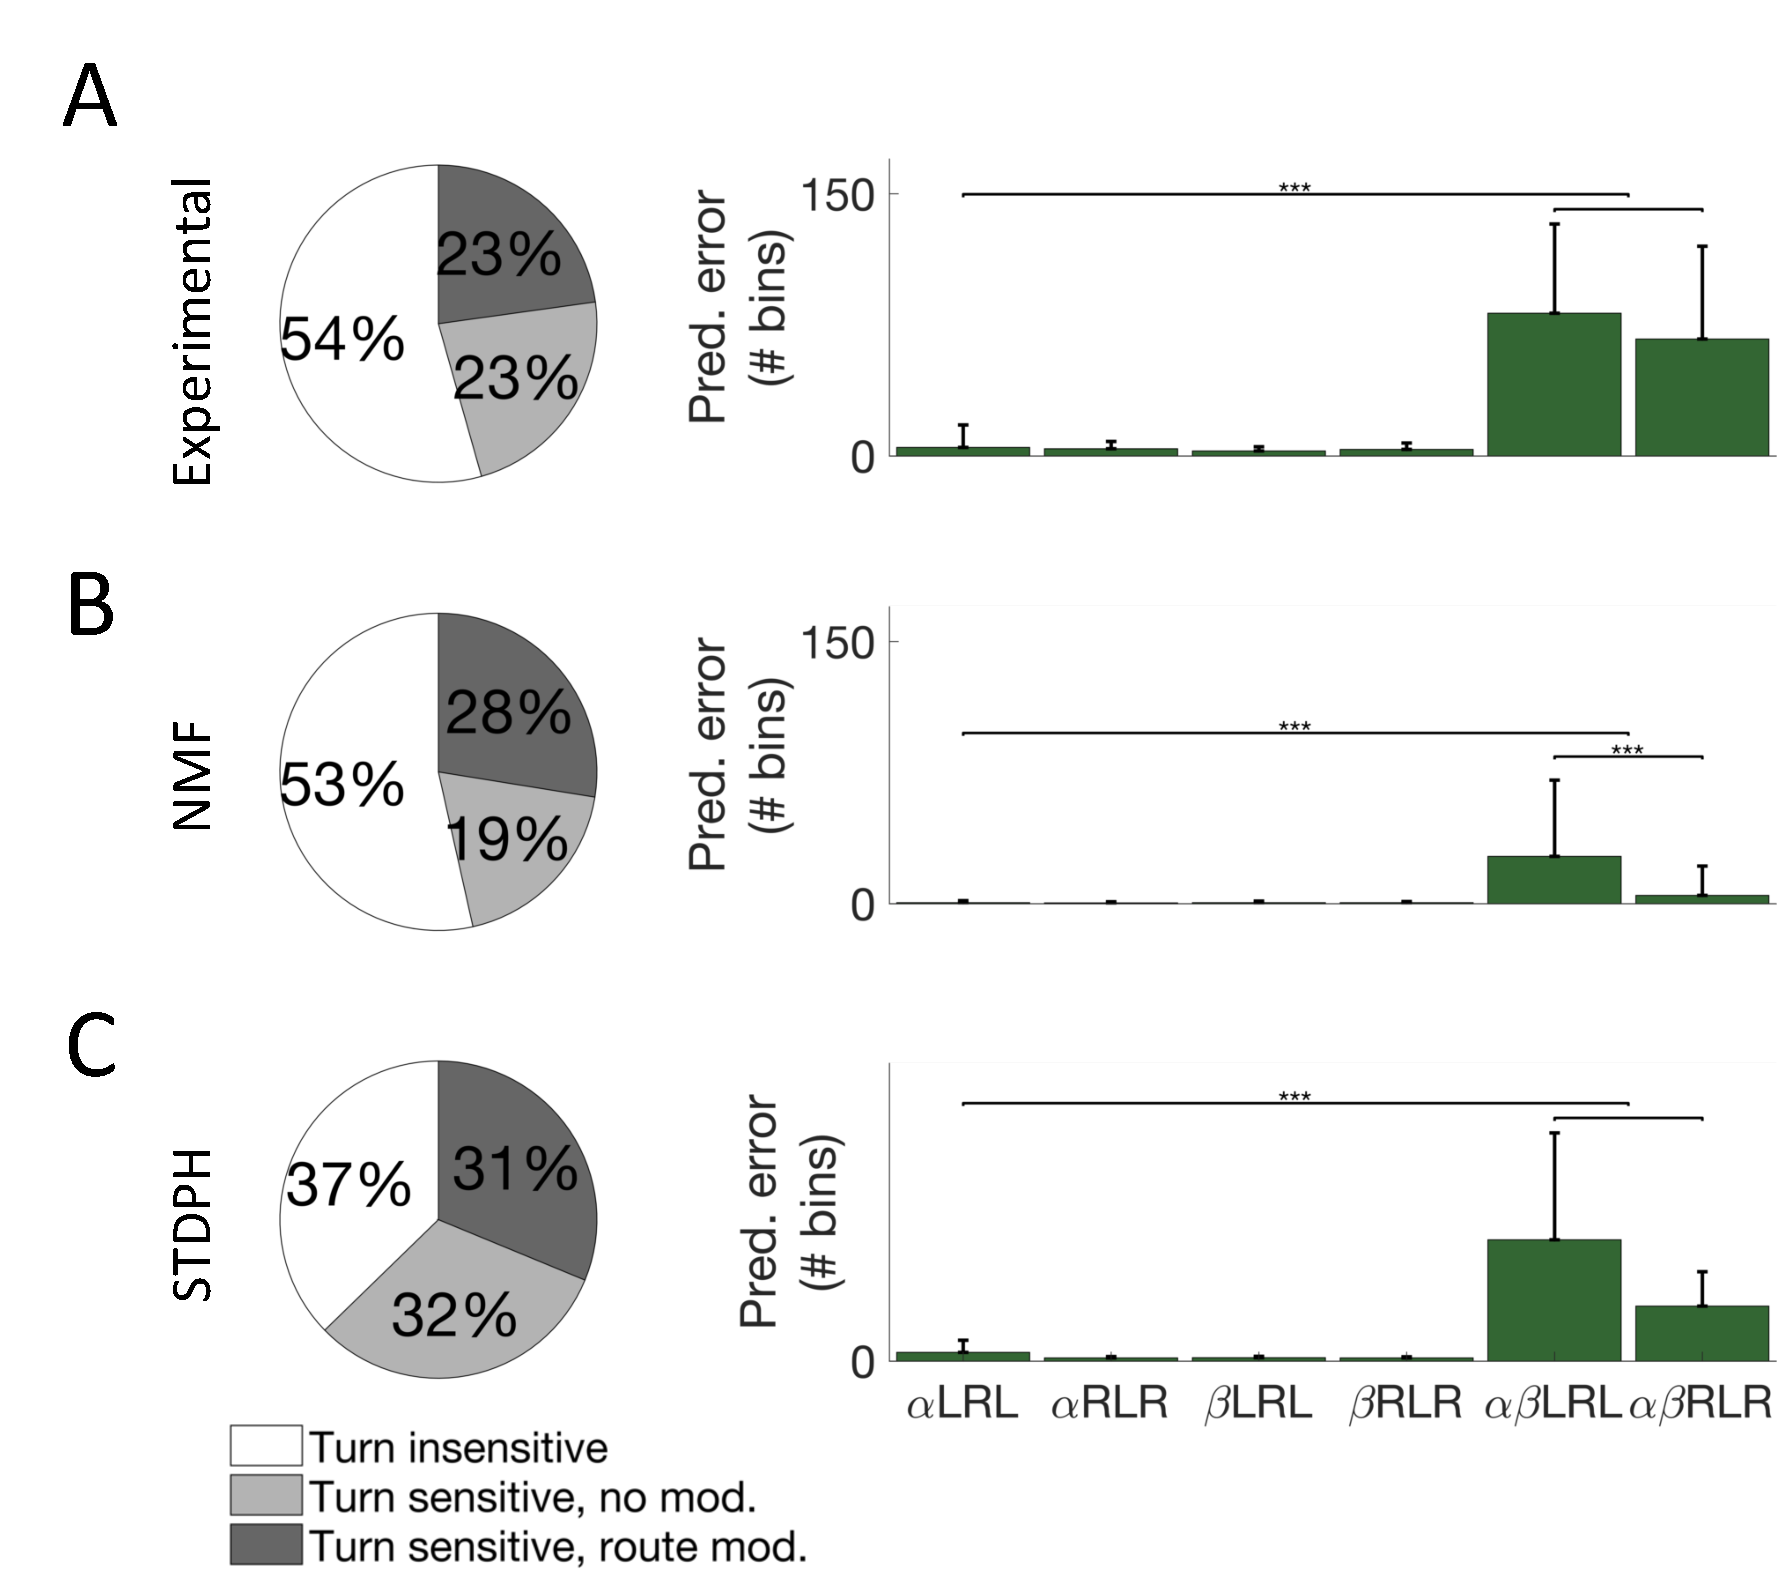
\includegraphics[width=\textwidth]{fig3}
    \caption{Functional neuron type distributions found in the dataset and produced by each model (left columns) and average error corresponding to positional ensemble reconstruction matrices (right columns). Separate allocentric positions of the track are represented by the symbols $\alpha$ and $\beta$. Reconstructions between the track positions are represented by $\alpha$$\beta$. There were two possible routes associated with each track: an outbound run consisting of a left-right-left (LRL) turn sequence and an inbound run consisting of a right-left-right (RLR) turn sequence. A) Experimental data from \cite{AlexanderNitz2015}. B) Simulated using NMF. C) Simulated by evolving STDPH parameters to fit experimental data from \cite{Rounds2016}.}
	\label{fig:NMF|RSC}
\end{figure} 



These findings lend credence to our proposal that \ac{NMF} and \ac{STDPH} 
are functionally equivalent.
Furthermore, the matrix \textbf{W} produced by \ac{NMF} when applied to the \ac{RSC} dataset was qualitatively similar to the synaptic weight matrices produced by 
simulations in which \ac{STDPH} was evolved to match the same dataset.

% This evidence suggests that there is merit to comparing
% synaptic weights generated with both \ac{NMF} and \ac{STDPH} to
% synaptic connections in the brain.
% In cases where synaptic weights from biological neurons are unavailable,
% simulated weight matrices could be used to advance theories of brain areas 
% with complicated neuronal responses
% (such as \ac{MSTd} or \ac{RSC});
% for example, by predicting neuronal responses to novel stimuli
% and simulating experimental perturbations.


% \ac{NSC} may have emerged as a general encoding strategy is because it can be approximated by certain forms of synaptic plasticity, such as \ac{STDPH}, under certain conditions. STDP, or spike-timing dependent plasticity,\emilyNote{this sentence implies STDPH -> NSC, but relationship could be other way: NSC->STDPH, so be careful with this idea here...}
% %is a learning mechanism by which synaptic weights are potentiated or depressed based on the precise spike times of pre- and post-synapic neurons. \ac{STDP} 
% is a learning mechanism that has been found in many brain regions and is generally assumed to take place in some form in every brain region. \emilyNote{much citations, very need} However, there may be many kinds of implementations of STDP in the brain that could also impose other statistical constraints in addition to nonnegativity. In a modified \ac{STDPH} learning rule, STDP is complemented by a homeostatic synaptic scaling mechanism that may give rise to a biologically realistic implementation of \ac{NMF}. In this view, a specific synaptic weight
% (i.e., an element in \textbf{W})
% is modulated depending on the activity of a presynaptic neuron over time
% (i.e., a row in \textbf{V})
% and the activity of a postsynaptic neuron over time
% (i.e., a column in $\mathbf{H}^T$).
% Here, the dimension that used to encompass a number of observations or stimuli $S$
% is now interpreted as time $t$.
% In this context, a row of \textbf{V} corresponds to a specific neuron's firing
% rate over time.
% Then the synaptic weight update rule of \ac{STDPH}
% is mathematically equivalent to an iteration step in \ac{NMF}
% (see \citep{Carlson2013} for a mathematical proof).
% This bestows upon a pre-postsynaptic neuron pair the ability to implement
% \ac{NMF} literally through learning.\emilyNote{more citations; maybe kris would have some} This process is exemplified in Figure \ref{fig:NMF|STDPH}. However, there are multiple kinds of homeostasis that may exist in the brain as well, which may change the nature of the statistical constraints on the pre- and post-synaptic neuron pairs. 

% Another reason might be the fact that \ac{NMF} can be approximated
% by \ac{STDPH} \citep{Carlson2013} (Box 2).

% \mikeNote{words whole para}
% \Ac{STDP} is a synaptic learning that modulates synaptic weights based on the
% precise firing of pre and postsynaptic neurons.
% \Ac{STDP} is ubiquitous in the brain (even in the adult brain, right),
% but it comes in many different forms.
% In one particular form, where \ac{STDP} is complemented with
% homeostatic synaptic scaling (which we refer to as \ac{STDPH}),
% it might be equivalent to \ac{NMF}.




% Do we ever actually define sparsity?


% % I'm pretty sure readers of a high-impact journal such as Trends in Neurosciences
% % have heard of lateral inhibition before...
% In addition to nonnegativity constraints,  sparsity in the neural code may be enforced by lateral inhibitory connections in which excited neurons  inhibit their neighbors such that only a few neurons remain sufficiently active in response to a stimulus, resulting in enhanced  sensory perception. This kind of anti-Hebbian learning can be implemented using the Oja learning rule, which can then be used to control the sparsity of the neural code to ensure a robust and fault-tolerant, but also energy efficient, encoding. % Also Oja approximates PCA and that may or may not be relevant. 
% This conception of STDPH as a biological implementation of NMF implies that the weight matrices generated by an NMF decomposition should be equivalent to those learned by biological neurons in the brain, and by artificial neurons in SNNs under STDPH. Comparing the weight matrix \textbf{W} from \ac{NMF} once again
% to empirical data makes it clear that there is a strong correspondence, and in the case of \ac{V1}, synaptic weights recovered with \ac{NMF} closely resemble biological weight matrices in cat \ac{V1}. Moreover, similar results can be achieved with \ac{STDPH}. 
% %iffy on this
% The structures of synaptic weight matrices in higher cortical regions are unknown;
% \mikeNote{Sure, we can make this prediction. But it is not testable}
% however, we predict that comparisons of the matrix W generated by NMF and STDPH for the simulated RSC data would resemble the actual weight matrix associated with RSC neurons in the biological brain.



% \subsection{Retina}
% \label{sec:evidence|vision|retina}

% % Using \ac{NMF} to explain single-trial spike trains in the retina \citep{Onken2016}.

% % Overview:
% % - A variety of methods were applied to retinal ganglion cells  in order to analyze their firing patterns
% % - These methods included spatiotemporal PCA, ICA, and NMF, but also included Tucker-2 factorization with orthogonality or non-negativity constraints (yielding orthogonal Tucker-2 and space-by-time NMF).
% % - Space-by-time methods were more accurately able to decompose firing patterns into modules or basis vectors
% % - While orthogonal Tucker-2 was able to pick up on variance between patterns that allowed for better reconstruction (more efficient and more robust), space-by-time NMF picked up on stereotyped patterns and resulted in more consistent and generalizable modules
% % - (What does this actually mean...?)

% %  Means that for patterns of stimuli with spatial and temporal components, space-by-time techniques will be better at representing the underlying structure of the data. But if patterns are inseparable in space/time, then you don't need tensor factorization.
% % ...So what happens in the brain? Presumably both kinds of stimuli are possible. Does the brain have both spatiotemporal coding and tensor factorization style coding? What circumstances dictate when which is employed, if so?

% In seeking a scalable way to analyze population codes for large numbers of neurons in both the spatial and temporal dimensions, researchers applied spatiotemporal PCA, ICA, and NMF to both simulated spike trains and neurophysiological spike trains recorded from the retinas of salamanders. %Poor axolotls. :( 
% They also applied tensor factorization methods with either orthogonality or non-negativity constraints. Tensor factorization is a method that decomposes data into separated spatial and temporal domains such that you get separate basis functions (or "modules") for each. This is important because neurons may vary their responses in the spatial domain based on location (neurons closer to one another may share common inputs, for example), and in the temporal domain by varying their response patterns over time.  By decomposing firing rate patterns into spatial and temporal domains separately, a neuron's spatial and temporal contributions to the population code can be elucidated \citep{Onken2016}.

% The different techniques were applied to simplified simulated datasets in order to test how well each technique could extract the 'ground truth' of a known pattern, either separable or inseparable in space and time. First the researchers applied techniques to simulated datasets with a high signal to noise ratio (SNR) that were separable in space and time, which should be easily distinguishable. Blocks of time in which neurons fired at 300 Hz were randomly interspersed amongst background firing of only 2 Hz.  In this case, only spatiotemporal NMF and space by time NMF (Tucker-2 tensor factorization with non-negativity constraints) could recover the underlying ground truth in the pattern.  Given a low SNR (30 Hz with background firing of 2 Hz) pattern that was separable in space and time, only space-by-time NMF was able to faithfully recover the underlying structure. When a pattern was inseparable in space and time (SNR was again 300 Hz to 2 Hz), space by time NMF could no longer recover the underlying blocks, but spatiotemporal NMF could, suggesting that NMF is a better technique for decomposing firing rate data into its fundamental components than PCA or ICA.

% The researchers also looked at the differences between the Tucker-2 factorization methods with non-negativity or orthogonality constraints in their ability to recover stereotyped and repeated firing patterns in the data. They found that orthogonal Tucker-2 factorization led to more robust and efficient representations, but they were overall less compact, and they did not lead to stable modules that recovered stereotyped firing patterns - instead, this kind of factorization yielded modules that were less consistent and seemed to extract differences in activation pattern across stimuli (as opposed to commonalities). The authors note that all other methods with statistical constraints had the same inconsistency, suggesting that non-negativity is the most promising constraint for extracting stereotyped firing.

% Following testing on known ground truth, the researchers recorded spikes from in vitro retinal ganglion cells  while the cells were exposed to natural images (either still photographs or videos). They then applied the Tucker-2 factorization methods (with orthogonality or non-negativity constraints) to the recorded datasets. The results were similar to the simulated data case; space-by-time NMF could decompose the data into compact and sparse representations with three temporal modules and eight spatial modules, while orthogonal Tucker-2 yielded four temporal modulates and sixteen spatial modules. While orthogonal Tucker-2 was also more accurate than space-by-time NMF for correctly decoding the activity, the resulting modules were again inconsistent and relied more on differences between patterns of firing rather than extracting similarities in firing pattern. The modules resulting from space-by-time NMF, on the other hand, were more consistent and more representative of an underlying stereotyped pattern of firing in addition to being a sparser and more compact representation. 
% % Is it important to talk about the contribution of first spike latency and redundancy in spatial/temporal coding?

%  The researchers used the time-only and space-only information to decode the natural images presented to the RGCs and found that decoding was far less accurate when information from the spatial dimension was missing, but only slightly less accurate (though still statistically significantly so) when information from the temporal domain was missing. Further experiments using first spike latency (in which space-by-time NMF was applied to an altered dataset where all spikes except the first one for each neuron and trial were deleted) suggested that information is carried redundantly by spike timing and rate coding, because decoding error was on par with space-by-time NMF under these conditions. Further investigations in which RGCs were shown flashed gratings in different orientations revealed that spike timing is especially important for discriminating fine differences in images that fall within the boundaries of a receptive field.
 
%  The authors conclude that NMF is a biologically plausible tool for spike train analysis (the outputs of NMF can be directly interpreted as synaptic weights, and they are highly generalizable), and that the reason it has been used in a limited number of cases may be due to the fact that spatiotemporal NMF does not perform robustly under certain conditions; specifically, conditions where there is significant overlap in firing patterns and when there is a low SNR. By using space-by-time NMF, these problems can be overcome, and also allows for the analysis of the spatiotemporal structure of neuronal firing patterns. We suggest that the good performance of space-by-time NMF in terms of its ability to extract a sparse and highly compact representation of the underlying structure of a neural code is further evidence that the brain may be employing similar methods for handling the high dimensionality of incoming stimuli. However, since not all patterns are separable in space and time, it is an open question how the brain might handle incoming information under such conditions.

% "The advantage of the non-negative decomposition was its ability to robustly find compact and directly interpretable firing patterns that occur across many different kinds of stimuli. These patterns can be used as basis functions to linearly build a set of code-words of firing patterns, complementing existing approaches [98, 99]. The shape of these firing patterns can thus be examined to provide important information about the structure of the neural code, for example to make hypotheses about the spatial and temporal resolution at which a neural code should be read out. As an example of the information that these modules may give, the structure of spatial modules extracted from RGCs suggests that informative patterns of simultaneous firing come from localized groups of neurons whose receptive fields are close together and that have similar stimulus tuning. "




% \subsection{Early visual cortex}
% \label{sec:evidence|vision|V1}
% % MB TODO

% A popular theory about early visual cortex function is that of sparse coding.

% Sparsity has been proposed as a general principle for the visual cortex. Barlow has argued for sparsity
% on the grounds that only a small proportion of neurons in V1 (and elsewhere??) fire in response to a
% given image and hence the response is ”sparse”. This is desirable for neurons because it means that only
% a few of them need to be active and expend energy (the brain consumes more energy than the rest of the
% body).

% The principle behind sparse coding is that the vision system has an over-complete set of basis functions.
% It tries to represent each image in terms of a small set of these functions. This over-completeness means
% that the the basis functions can be tuned to interesting features of the image. As mentioned above, the
% sparsity principle can also be used to learn receptive fields from natural images (refs!!).

% This sparsity criteria was developed by Olshausen and Field as a way to learn receptive fields of
% neurons \citep{OlshausenField1996}. It gives a reconstruction criteria that can be extended to multiple images and used to learn receptive fields.

% This results in receptive field models which are similar to those measured \citep{OlshausenField1996}. Note that similar
% receptive fields can be obtained by assuming a similar model for the image, see equation (7), but imposing
% different assumptions on the form of the si
% . In particular, independent component analysis (ICA) gives
% similar receptive field models \citep{vanHateren1998}.
% \cite{Hyvarinen2010} explained this by showing that both types of models –
% L1 sparsity and \ac{ICA} – both encourage that the $s_i$ are strongly peaked at 0, 
% but can occasionally have
% large non-zero values (this contrasts with the Gaussian model – e.g. pseudo-inverse – where the 
% $s_i$ are strongly discouraged from taking large values).



% % Topographic NMF: \url{http://www.mitpressjournals.org/doi/pdf/10.1162/neco.2009.03-08-722}
% % It seems like they're adding space to the NMF computation, which might make this kind of similar to the space-by-time NMF algorithm discussed in the retina paper? Am I thinking about that correctly? -Emily






% \subsection{Audition}
% \url{https://www.ncbi.nlm.nih.gov/pmc/articles/PMC4747712/}
% Wondering if NMF could explain the feature composition

% \subsection{Speech}
% S. Zayd Enam, Michael R. DeWeese: Spectro-Temporal Models of Inferior Colliculus Neuron Receptive Fields 
% Sparse codes for speech spectrograms qualitatively match properties of receptive fields of Inferior Colliculus (ICC) neurons. We find sparse codes of speech-spectrograms are well described by one of four models and we find that these models also fit ICC spectro-temporal receptive fields (STRF) well. Further, our models are able to express time-frequency inseparable receptive fields (e.g. frequency sweeps) that previous models were unable to satisfactorily describe. Our models allow the accurate characterization of high-dimensional STRFs with more natural parameterizations of the neuron's behavior. \emilyNote{Not sure we'd want to cite this paper? "To determine STRF model classes we first fit model classes to the sparse codes of speech-spectrograms using non-linear least squares methods"}


% \subsection{Olfaction}

% % Structure this as...
% % 1) There are lots of possible odor combinations and sparse ensemble of neurons to encode them
% % 2) The sparsity of the olfactory code is poor in information and metabolically costly, so functional significance is unclear
% % 3)  Granule cells may complement the code of the mitral cells because they are sparse/incomplete representations
% % 4) This might result in 'explaining away' approach by this system as described in the SNN paper, which was able to detect combinations of odorants very accurately
% % 5) Brief description of causal inference in spiking via explaining away and how it relates to NMF?


% Check this Drugowitsch paper:
% Causal Inference and Explaining Away in a Spiking Network
% Rubén Moreno-Bote \& Jan Drugowitsch, Scientific Reports
% \url{https://www.nature.com/articles/srep17531}

% Also Koulakov and Rinberg:
% Sparse incomplete representations: A novel role for olfactory granule cells
% \url{https://pdfs.semanticscholar.org/ed52/1b318aa68fe8ec71fb9a84d5e577130c6893.pdf}

% It's \emph{almost} doing \ac{NMF},
% and suggests that such a computation might underlie odor classification.

% Antennae -> antennal lobe -> mushroom body (Kenyan cell)
% only 34 output neurons for odor classification
% any given odor activates a unique and sparse ensemble of kenyan cells

% From Graziano \& Aflalo: In this review, the authors suggest that at least some sectors of the cortex do not have a simple global ordering and are better understood as a result of a reduction of a highdimensional space onto the cortical sheet. The cortical motor system may be an example of this phenomenon. The authors discuss a model of the lateral motor cortex in which a reduction of many parameters onto a simulated cortical sheet results in a complex topographic pattern that matches the actual monkey motor cortex in surprising detail. \citep{GrazianoAflalo2007} Source:

% \url{https://www.princeton.edu/~graziano/neuroscientist_07.pdf}
% \url{http://ieeexplore.ieee.org/document/7229368}


% % \subsection{Somatosensory cortex}
% % % MB probably cut...

% % Chapin \& Nicolelis (1999). Journal of Neuroscience Methods. Principal component analysis of neuronal ensemble activity reveals multidimensional somatosensory representations.
% % Recorded neurons from rat somatosensory cortex and applied PCA to the data. Found multidimensional somatosensory receptive fields.
% % From abstract: "The fact that this transformation is mathematically equivalent to the general Hebb algorithm in linear neural networks provided a major rationale for performing it here on data from real neuronal ensembles."

